

\documentclass[12pt]{article}

%\pagestyle{empty} 
\usepackage{amsmath}
\usepackage{algpseudocode}
\usepackage{algorithm}
\usepackage[english]{babel}
\usepackage{amsthm}
\usepackage{amssymb}
\usepackage{color}
\usepackage{graphicx}
\usepackage{epsfig}

\newcommand{\vs}{\vspace{2mm}}
\newcommand{\ls}{\vspace{5mm}} 

\newcommand{\ms}{\vspace{3mm}}
\newcommand{\bc}{\begin{center}}
\newcommand{\ec}{\end{center}}
\newcommand{\sm}{\small}
\newcommand{\hs}{\hspace{10mm}}
\newcommand{\ha}{\hspace{1mm}}
\newcommand{\bo}{\rule{2mm}{3mm}}
\textheight=680pt
\textwidth=460pt
\hoffset=-50pt
\voffset=-50pt
%\topmargin=-0.5in
%\textheight=10in
%\oddsidemargin=0.125in
%\evensidemargin=0.125in
%\textwidth=7.5in
\begin{document}
\bc\ 
 { \bf  Homework  1 (50 points)}  Due: September 13, 2024 11:59 pm\\
 { \bf COMPSCI 733: Advanced Algorithms and Designs } \\ 
 { \bf Benzon Carlitos Salazar (salazarbc24@uww.edu) } 
\ec\  
\ls\

\noindent{\bf Documentation:} (5 points)
Type your solutions using Latex \\
(www.overleaf.com or https://www.latex-project.org/ ). Submit your solutions (pdf is enough)  to Canvas. 




\vs\

\noindent{\bf Problem 1: (15 points)}
Assume we have a one dimensional array of real numbers with $A.length = n$ and indices, $1, 2, \ldots, n$.
In the code for InsertionSort  shown below, the outer loop index $j$ goes from 2 to $n$, and the inner index i of the while loop goes “backward”. 

\begin{algorithm}
\caption{INSERTION-SORT-FORWARD(A)}
\begin{algorithmic}[1]
\For {$j=2$ to $n$}
\State{$key=A[j]$}
\State{//Insert $A[j]$ into the sorted sequence $A[1,\ldots,j-1].$}
\State{$i=j-1$}
\While{$i > 0$ and $A[i] > key$} 
  State{$A[i+1]=A[i]$} 
    \State $i = i-1$
\EndWhile
\State {$A[i+1] = key$}
\EndFor
\end{algorithmic}
\end{algorithm}

\begin{itemize}
 \item[(a)] Write a version of the pseusocode for InsertionSortBackward where the outer index j goes “backward”, and the inner index i goes “forward”.  

\begin{algorithm}
\caption{INSERTION-SORT-BACKWARD(A)}
\begin{algorithmic}[1]
\For {$j = n-1$ to $1$}
    \State{$key = A[j]$}
    \State{// Insert $A[j]$ into the sorted sequence $A[j+1, \ldots, n]$}
    \State{$i = j + 1$}
    \While{$i \leq n$ and $A[i] < key$}
        \State{$A[i-1] = A[i]$}
        \State{$i = i + 1$}
    \EndWhile
    \State{$A[i-1] = key$}
\EndFor
\end{algorithmic}
\end{algorithm}

\item[(b)] Prove that your program (InsertionSortBackward)is correct.
See CLRS Chapter 2 and the given "ProgramCorrectness.pptx" slides.

Steps:
\begin{itemize}
\item[1.]	 Write a loop invariant.
\item[2.]	Show Initialization holds.
\item[3.]Show Maintenance  holds.
\item[4.]	Show Termination holds.
\end{itemize}
\end{itemize}

\textbf{Loop Invariant:} \\
At the start of each iteration of the outer loop (with index $j$), the subarray $A[j+1, \ldots, n]$ consists of the elements that were originally in those positions, but sorted in increasing order.

\vs
- Before the iteration, the subarray $A[j+1]$ to $A[n]$ is sorted. \\
- During the iteration, $A[j]$ is inserted into its correct position within this sorted subarray. \\
- After the iteration, the subarray from $A[j]$ to $A[n]$ is sorted.

\vs
\textbf{Step 1: Initialization} \\
We show that the loop invariant holds before the first iteration of the outer loop.

- \textbf{Before the first iteration}, the outer loop starts with $j = n-1$, meaning that the subarray $A[n]$ (which consists of a single element) is trivially sorted. \\
- Thus, the loop invariant holds initially, since a single element is always sorted.

\vs
\textbf{Step 2: Maintenance} \\
We show that if the loop invariant holds before the current iteration of the outer loop, it will hold after the iteration as well.

- \textbf{During the iteration}, the key $A[j]$ is compared with the elements in $A[j+1]$ through $A[n]$, which are sorted. \\
- The inner loop shifts elements to the left as long as they are smaller than the key, and once the correct position is found, the key is inserted. \\
- \textbf{After the iteration}, the subarray $A[j, \ldots, n]$ is sorted because the key is now in its proper position within the previously sorted subarray.
- Hence, the loop invariant continues to hold.

\vs
\textbf{Step 3: Termination} \\
We show that when the outer loop terminates, the entire array is sorted.

- \textbf{Termination occurs when} $j = 0$. At this point, the loop invariant tells us that the subarray $A[1, \ldots, n]$ is sorted. \\
- Since $j = 0$ corresponds to the entire array, the whole array is now sorted.

\vs\
\pagebreak

\noindent{\bf Problem 2: (15 points) }

A tree is a simple connected graph with no cycles.

\begin{figure}[!h]
\centering
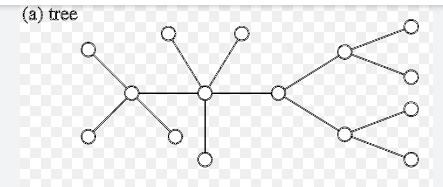
\includegraphics[scale=1]{TreeExample.jpg}
\caption{}
\label{fig1}
\end{figure}

Use the mathematical induction steps given in the following template to prove that a tree with $n$ vertices has exactly $n-1$ edges for all $n \geq 1$.

\vs

\noindent{\bf Induction proof template:}

\noindent{$P(n):$} A tree with $n$ vertices has exactly $n-1$ edges.
\ls

\noindent{\em Prove:} $P(n)$ is true for all $n \geq 1$.

\vs
\begin{proof} (By induction on $n$)
    \begin{itemize}
    \item \textbf{Base Case:} \\
    For $n = 1$, the tree consists of a single vertex with no edges. Therefore, a tree with $n = 1$ vertex has $1-1 = 0$ edges, which satisfies $P(1)$.

    \item \textbf{Inductive Hypothesis:} \\
    Assume that for $n = k$ (for some arbitrary $k \geq 1$), any tree with $k$ vertices has exactly $k-1$ edges. This is our inductive hypothesis.
    
    \item \textbf{Inductive Step:} \\
    We must show that $P(k+1)$ is true, i.e., a tree with $k+1$ vertices has exactly $(k+1) - 1 = k$ edges. \\
    Consider any tree with $k+1$ vertices. Since a tree is connected and acyclic, we can remove a leaf vertex (a vertex with degree 1), along with its corresponding edge. After removing this vertex and its edge, the remaining graph is still a tree with $k$ vertices. By the inductive hypothesis, this tree has $k-1$ edges. Adding the removed edge back to the graph, we now have $k$ edges for the tree with $k+1$ vertices.

    \item \textbf{Conclusion:} \\
    Therefore, by the principle of mathematical induction, $P(n)$ is true for all $n \geq 1$, and a tree with $n$ vertices has exactly $n-1$ edges.
    \end{itemize}
\end{proof}

\noindent{\bf Problem 3: (15 points)}

Use strong induction to show that every positive integer $n$ can be written as a sum of distinct powers of two, that is, as a sum of a subset of the integers $2^0 , 2^1 , 2^2 …,$ and so on  i.e., $1=2^0 , 2=  2^1 , 3=2^0+ 2^1, 4=2^2 , ... $. [Hint: For the inductive step, separately consider the cases where $k + 1$ is even and where $k+1$ is odd. When it is even, note that $(k + 1)/2$ is an integer.]
\vs\

\noindent{\bf Strong induction proof template:}

\noindent{$P(n):$}  Every positive integer $n$ can be written as a sum of distinct powers of two.
\ls\

\noindent{\em Prove:} $P(n)$ is true for all $n \geq 1$.
\vs\

\begin{proof} (By strong induction on $n$)

    \begin{itemize}
    
    \item \textbf{Base Case:} \\
    For $n = 1$, we have $1 = 2^0$, which is a sum of distinct powers of two. Hence, the base case holds for $n = 1$.
    
    \item \textbf{Strong Inductive Hypothesis:} \\
    Assume that for all integers $n = 1, 2, \ldots, k$, each of these numbers can be written as a sum of distinct powers of two. We will now show that $P(k+1)$ is true.

    \item \textbf{Inductive Step:} \\
    We consider two cases for $k+1$:
    
    \begin{itemize}
    
    \item \textbf{Case 1:} $k + 1$ is odd. \\
    If $k + 1$ is odd, we can write it as $k + 1 = 2m + 1$ for some integer $m$. By the strong inductive hypothesis, $m$ can be written as a sum of distinct powers of two, say $m = 2^{a_1} + 2^{a_2} + \dots + 2^{a_r}$. Therefore,
    \[
    k + 1 = 2m + 1 = 2(2^{a_1} + 2^{a_2} + \dots + 2^{a_r}) + 2^0.
    \]
    Hence, $k + 1$ can be written as a sum of distinct powers of two.
    
    \item \textbf{Case 2:} $k + 1$ is even. \\
    If $k + 1$ is even, we can write it as $k + 1 = 2m$ for some integer $m$. By the strong inductive hypothesis, $m$ can be written as a sum of distinct powers of two, say $m = 2^{a_1} + 2^{a_2} + \dots + 2^{a_r}$. Therefore,
    \[
    k + 1 = 2m = 2(2^{a_1} + 2^{a_2} + \dots + 2^{a_r}),
    \]
    which is also a sum of distinct powers of two.
    
    \end{itemize}
    
    In both cases, we have shown that $k + 1$ can be written as a sum of distinct powers of two.

    \item \textbf{Conclusion:} \\
    Therefore, by the principle of strong induction, $P(n)$ is true for all $n \geq 1$, meaning that every positive integer $n$ can be written as a sum of distinct powers of two.
    
    \end{itemize}
    
\end{proof}


\end{document}

